%%%%%%%%%%%%%%%%%%%%%%%%%%%%%%%%%%%%%%%%%
% Professional Mathematical Presentation Template
% 
% This template uses the beamer class with the Madrid theme
% and a custom color scheme for a clean, professional look
% that works well with mathematical content.
%%%%%%%%%%%%%%%%%%%%%%%%%%%%%%%%%

\documentclass[aspectratio=169]{beamer} % 16:9 aspect ratio (modern)

% Theme settings
\usetheme{Madrid}
\usecolortheme{default}


\definecolor{primcolor}{RGB}{25,50,100} % Dark blue
\setbeamercolor{structure}{fg=primcolor}
\setbeamercolor{frametitle}{bg=primcolor!15, fg=primcolor}
\setbeamercolor{title}{fg=white} % White title text for contrast
\setbeamercolor{subtitle}{fg=white} % White subtitle text
\setbeamercolor{author}{fg=primcolor} % White author text
\setbeamercolor{date}{fg=primcolor} % White date text
\setbeamercolor{institute}{fg=primcolor} % White institute text

% Font settings
\usefonttheme{professionalfonts}
\usefonttheme{serif}

% Package imports
\usepackage{amsmath, amsfonts, amssymb, amsthm} % Math packages
\usepackage{mathtools} % Enhanced math tools
\usepackage{bm} % Bold math symbols
\usepackage{graphicx} % For images
\usepackage{booktabs} % Professional tables
\usepackage{tikz} % For diagrams
\usetikzlibrary{arrows, positioning, matrix, decorations.pathreplacing}

% Use beamer's theorem styles
\setbeamertemplate{theorem}[ams style]
\setbeamertemplate{theorems}[numbered]


% Remove navigation symbols
\setbeamertemplate{navigation symbols}{}

% Custom footer
\setbeamertemplate{footline}{
  \leavevmode%
  \hbox{%
  \begin{beamercolorbox}[wd=.333333\paperwidth,ht=2.25ex,dp=1ex,center]{author in head/foot}%
    \usebeamerfont{author in head/foot}\insertshortauthor
  \end{beamercolorbox}%
  \begin{beamercolorbox}[wd=.333333\paperwidth,ht=2.25ex,dp=1ex,center]{title in head/foot}%
    \usebeamerfont{title in head/foot}\insertshorttitle
  \end{beamercolorbox}%
  \begin{beamercolorbox}[wd=.333333\paperwidth,ht=2.25ex,dp=1ex,right]{date in head/foot}%
    \usebeamerfont{date in head/foot}\insertshortdate{}\hspace*{2em}
    \insertframenumber{} / \inserttotalframenumber\hspace*{2ex} 
  \end{beamercolorbox}}%
  \vskip0pt%
}

% Title information
\title[DRL]{Deep Reinforcement Learning can promote sustainable human behaviour in common-pool resource problems}
\subtitle{Koster et al. 2025}
\author[Longye]{Longye Tian \\ \texttt{longye.tian@anu.edu.au}}
\institute[ANU]{Australian National University\\ School of Economics}
\date{March 27th, 2025}
\DeclareFontFamily{U}{mathx}{\hyphenchar\font45}
\DeclareFontShape{U}{mathx}{m}{n}{
      <5> <6> <7> <8> <9> <10>
      <10.95> <12> <14.4> <17.28> <20.74> <24.88>
      mathx10
      }{}
\DeclareSymbolFont{mathx}{U}{mathx}{m}{n}
\DeclareMathSymbol{\bigtimes}{1}{mathx}{"91}

\begin{document}

% Title frame
\begin{frame}
  \titlepage
\end{frame}

% Outline frame
\begin{frame}{Outline}
  \tableofcontents
\end{frame}

\section{Motivation}
\begin{frame}{Motivation}
\begin{itemize}
    \item \textbf{Common-pool resource problem:} How to allocate public resources to achieve sustainability?
    \item \textbf{Social dilemma:} Each recipient can choose to:
    \begin{itemize}
        \item Reciprocate (for common good)
        \item Keep proceeds selfishly (for individual benefit)
    \end{itemize}
    \item \textbf{Challenge:} Agents are not allowed to communicate, contract, or sanction each other
    \item \textbf{Goal:} Find a resource allocation rule that encourages reciprocation
    \item \textbf{Metrics of success:} Equality, sustainability, and quality of life
\end{itemize}
\end{frame}

\begin{frame}{Game Setup: The Iterated Trust Game}
\begin{center}
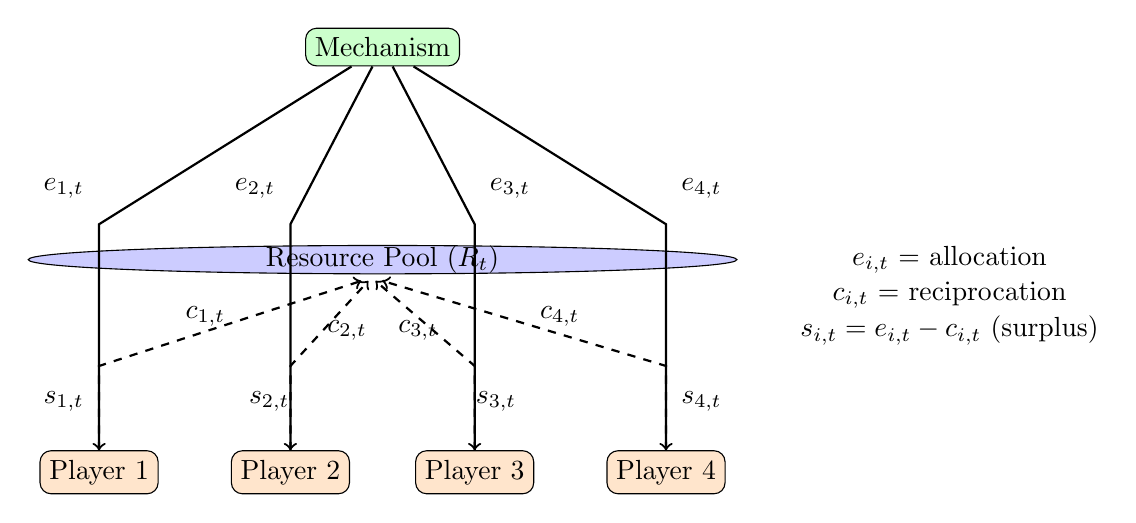
\begin{tikzpicture}[scale=0.9]
    % Pool
    \draw [fill=blue!20] (0,0) ellipse (5cm and 0.2cm);
    \node at (0,0) {Resource Pool ($R_t$)};
    
    % Players
    \node[draw, rounded corners, fill=orange!20] (p1) at (-4,-3) {Player 1};
    \node[draw, rounded corners, fill=orange!20] (p2) at (-1.3,-3) {Player 2};
    \node[draw, rounded corners, fill=orange!20] (p3) at (1.3,-3) {Player 3};
    \node[draw, rounded corners, fill=orange!20] (p4) at (4,-3) {Player 4};
    
    % Mechanism
    \node[draw, rounded corners, fill=green!20] (m) at (0,3) {Mechanism};
    
    % Allocation arrows
    \draw[->, thick] (m) -- (-4,0.5) -- (p1);
    \draw[->, thick] (m) -- (-1.3,0.5) -- (p2);
    \draw[->, thick] (m) -- (1.3,0.5) -- (p3);
    \draw[->, thick] (m) -- (4,0.5) -- (p4);
    
    % Reciprocation arrows
    \draw[->, thick, dashed] (p1) -- (-4,-1.5) -- (-0.3,-0.3);
    \draw[->, thick, dashed] (p2) -- (-1.3,-1.5) -- (-0.2,-0.3);
    \draw[->, thick, dashed] (p3) -- (1.3,-1.5) -- (-0.1,-0.3);
    \draw[->, thick, dashed] (p4) -- (4,-1.5) -- (0,-0.3);
    
    % Labels
    \node at (-4.5,1) {$e_{1,t}$};
    \node at (-1.8,1) {$e_{2,t}$};
    \node at (1.8,1) {$e_{3,t}$};
    \node at (4.5,1) {$e_{4,t}$};
    
    \node at (-2.5,-0.8) {$c_{1,t}$};
    \node at (-0.5,-1) {$c_{2,t}$};
    \node at (0.5,-1) {$c_{3,t}$};
    \node at (2.5,-0.8) {$c_{4,t}$};

    \node at (-4.5,-2) {$s_{1,t}$};
    \node at (-1.6,-2) {$s_{2,t}$};
    \node at (1.6,-2) {$s_{3,t}$};
    \node at (4.5,-2) {$s_{4,t}$};
    
    % Legend
    \node at (8,0) {$e_{i,t}$ = allocation};
    \node at (8,-0.5) {$c_{i,t}$ = reciprocation};
    \node at (8,-1) {$s_{i,t} = e_{i,t} - c_{i,t}$ (surplus)};
\end{tikzpicture}
\end{center}
\end{frame}


\begin{frame}{The Problem in Context}
\begin{itemize}
    \item \textbf{Real-world examples:}
    \begin{itemize}
        \item Government providing startup loans to companies
        \item Employers allocating resources to employees
        \item Sustainable stewardship of shared resources
        \item Financial endowments, forests, fisheries, global environment
    \end{itemize}
    \item \textbf{Prior approaches} focused on self-organization mechanisms:
    \begin{itemize}
        \item Communication between players ("cheap talk")
        \item Ability to sanction uncooperative members
        \item Voting mechanisms for exclusion of free riders
    \end{itemize}
    \item \textbf{This paper:} How can a central authority allocate resources effectively \textit{without} these self-organization mechanisms?
\end{itemize}
\end{frame}

\section{Big Picture}

\begin{frame}{Main Idea}
\begin{enumerate}
    \item Collect data from human players under various allocation mechanisms
    \item \textcolor{blue}{Train neural networks (behavioral clones) to imitate human behaviors}
    \item Use these behavioral clones to create more data for RL agents to design a mechanism 
    \item Adopt that RL-based mechanism with real humans to validate its performance
    \item Interpret the RL-based mechanism to create an understandable heuristic
\end{enumerate}

\begin{center}
\textbf{Key innovation:} Using deep RL to discover top-down resource allocation mechanisms that promote sustainable behavior without requiring communication between players
\end{center}
\end{frame}

\begin{frame}{The Game Structure}
\begin{itemize}
    \item \textbf{Setup:} 4 players, resource pool initialized at 200 units
    \item \textbf{Each round:}
    \begin{itemize}
        \item Social planner allocates endowments ($e_{i,t}$) to players from pool
        \item Players choose how much to reciprocate ($c_{i,t}$)
        \item Reciprocated amount grows by factor $r = 0.4$ (40\%)
        \item Player keeps remainder as surplus ($s_{i,t} = e_{i,t} - c_{i,t}$)
    \end{itemize}
    \item \textbf{Pool dynamics:} 
    \begin{itemize}
        \item Updated as: $R_t = \min(R_0, R_{t-1} + \Delta R_t)$
        \item Where $\Delta R_t = -\sum_i e_{i,t} + (1+r)\sum_i c_{i,t}$
    \end{itemize}
    \item \textbf{Game continues} until pool depleted or maximum rounds reached
\end{itemize}
\end{frame}

\section{Methodology}

\begin{frame}{Research Pipeline}
\begin{enumerate}
    \item \textbf{Initial baseline mechanisms:}
    \begin{itemize}
        \item Equal allocation ($w = 1$): Everyone gets the same share
        \item Proportional allocation ($w = 0$): Share based on past contribution
        \item Mixed allocation ($w = 0.5$): Combination of both approaches
    \end{itemize}
    \item \textbf{Data collection:} Human players interact with these baselines
    \item \textbf{Behavioral cloning:} Train neural networks to mimic human behavior
    \item \textbf{Train RL agent:} Using simulated economy with behavioral clones
    \item \textbf{Evaluate:} Test RL agent with new human participants
    \item \textbf{Analyze and interpret:} Derive explainable mechanism
\end{enumerate}
\end{frame}


\begin{frame}{Behavioral Cloning}
\begin{itemize}
    \item \textbf{Concept:} Create neural networks that imitate human players
    \item \textbf{Architecture:}
    \begin{itemize}
        \item Recurrent neural networks with GRU (Gated Recurrent Units)
        \item Inputs: Current offers to all players, previous contributions, current pool size
        \item Outputs: Predicted player contribution
    \end{itemize}
    \item \textbf{Training:} Supervised learning on human gameplay data
    \item \textbf{Validation:} Comparing behavior to human players across multiple metrics
    \item \textbf{Benefits:}
    \begin{itemize}
        \item Allows rapid experimentation with different mechanisms
        \item Creates a "sandbox economy" for training the RL agent
        \item Enables prediction of outcomes for new mechanisms
    \end{itemize}
\end{itemize}
\end{frame}

\begin{frame}{RL Agent Architecture}
\begin{itemize}
    \item \textbf{Graph Neural Networks (GNNs)} for resource allocation policy:
    \begin{itemize}
        \item Ensures uniform opening move (equal first offers)
        \item Provides equivariance to permutation in player ordering
    \end{itemize}
    \item \textbf{Memory component} using Gated Recurrent Units:
    \begin{itemize}
        \item Allows mechanism to condition on history within episode
        \item Enables complex temporal policies
    \end{itemize}
    \item \textbf{Objective function:} Maximize aggregate surplus across all players
    \begin{itemize}
        \item $\max \sum_{t=0}^{T=40}\sum_{i=1}^{N=4}(e_{i,t} - c_{i,t})$
    \end{itemize}
    \item \textbf{Training environment:} Interactions with behavioral clones
\end{itemize}
\end{frame}

\section{Results}

\begin{frame}{Baseline Mechanism Results}
\begin{columns}
\begin{column}{0.6\textwidth}
\textbf{Equal Allocation ($w = 1$):}
\begin{itemize}
    \item Low overall surplus
    \item Low inequality (Gini coefficient ≈ 0.1)
    \item Rapid collapse of reciprocation
    \item Only 5\% of games sustained to end with all players
\end{itemize}

\textbf{Proportional Allocation ($w = 0$):}
\begin{itemize}
    \item Higher surplus but high inequality (Gini ≈ 0.4)
    \item Players often fall into "poverty traps"
    \item 60\% of games sustained to end, but never with all players
    \item Often results in monopolistic situations
\end{itemize}
\end{column}
\begin{column}{0.4\textwidth}
\begin{center}
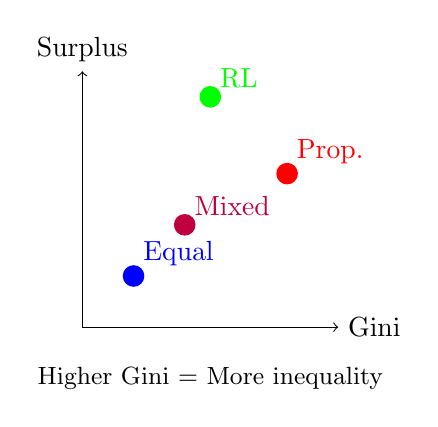
\begin{tikzpicture}[scale=0.65]
    % Axes
    \draw[->] (0,0) -- (5,0) node[right] {Gini};
    \draw[->] (0,0) -- (0,5) node[above] {Surplus};
    
    % Data points
    \filldraw[blue] (1,1) circle (0.2) node[above right] {Equal};
    \filldraw[purple] (2,2) circle (0.2) node[above right] {Mixed};
    \filldraw[red] (4,3) circle (0.2) node[above right] {Prop.};
    \filldraw[green] (2.5,4.5) circle (0.2) node[above right] {RL};
    
    % Annotations
    \node[align=left, font=\small] at (2.5,-1) {Higher Gini = More inequality};
\end{tikzpicture}
\end{center}
\end{column}
\end{columns}
\end{frame}

\begin{frame}{RL Agent Performance}
\begin{columns}
\begin{column}{0.6\textwidth}
\textbf{RL Agent results:}
\begin{itemize}
    \item 150\% greater surplus than highest baseline
    \item Moderate inequality (Gini ≈ 0.2)
    \item 65\% of games sustained to the end
    \item 55\% of games sustained with all four players
    \item Maintained more active players than other mechanisms
\end{itemize}

\textbf{Key achievement:} Under RL mechanism, games with higher surplus were more egalitarian (negative correlation) - unlike baselines
\end{column}
\begin{column}{0.4\textwidth}
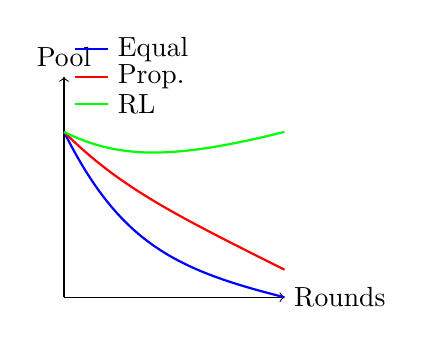
\begin{tikzpicture}[scale=0.7]
    % Pool size over time
    \draw[->] (0,0) -- (4,0) node[right] {Rounds};
    \draw[->] (0,0) -- (0,4) node[above] {Pool};
    
    % Different trajectories
    \draw[blue, thick] (0,3) .. controls (1,1) and (2,0.5) .. (4,0);
    \draw[red, thick] (0,3) .. controls (1,2) and (2,1.5) .. (4,0.5);
    \draw[green, thick] (0,3) .. controls (1,2.5) and (2,2.5) .. (4,3);
    
    % Legend
    \draw[blue, thick] (0.2,4.5) -- (0.8,4.5); \node[right] at (0.8,4.5) {Equal};
    \draw[red, thick] (0.2,4) -- (0.8,4); \node[right] at (0.8,4) {Prop.};
    \draw[green, thick] (0.2,3.5) -- (0.8,3.5); \node[right] at (0.8,3.5) {RL};
\end{tikzpicture}
\end{column}
\end{columns}
\end{frame}

\begin{frame}{What Made the RL Agent Successful?}
\begin{enumerate}
    \item \textbf{Conditional allocation based on pool size:}
    \begin{itemize}
        \item More egalitarian when resources abundant
        \item More selective when resources scarce
    \end{itemize}
    
    \item \textbf{Temporary exclusion strategy:}
    \begin{itemize}
        \item Sanctions defectors briefly (~1-5 rounds)
        \item Makes generous offers upon re-inclusion
        \item Similar to "tit-for-two-tats" or "generous tit-for-tat"
    \end{itemize}
    
    \item \textbf{Forward-looking offers:}
    \begin{itemize}
        \item Offers predict reciprocation rather than following it
        \item "Coaxes" players into reciprocating with strategic offers
    \end{itemize}
\end{enumerate}
\end{frame}

\begin{frame}{Creating an Explainable Mechanism}
\begin{itemize}
    \item \textbf{Challenge:} RL agent policy is effective but not easily interpretable
    
    \item \textbf{Solution:} Create simpler mechanism that approximates RL behavior
    \begin{itemize}
        \item Interpolating baseline with varying $w$ parameter: $w = (R/200)^k$
        \item When pool is low: more proportional allocation
        \item When pool is high: more equal allocation
        \item Optimal exponent $k = 22$ (determined empirically)
    \end{itemize}
    
    \item \textbf{Results:}
    \begin{itemize}
        \item Comparable surplus to RL agent
        \item Lower Gini coefficient (more equal)
        \item More popular with human participants
        \item Judged as fairer, more understandable, and more cooperative
    \end{itemize}
\end{itemize}
\end{frame}

\begin{frame}{Interpolating Baseline Performance}
\begin{columns}
\begin{column}{0.55\textwidth}
\begin{itemize}
    \item \textbf{Formula:} $w = (R/200)^{22}$
    \item \textbf{Properties:}
    \begin{itemize}
        \item Roughly proportional unless pool almost full
        \item Provides similar temporary exclusion pattern to RL
        \item Gives excluded players meaningful offers upon re-inclusion
    \end{itemize}
    \item \textbf{Human preferences:}
    \begin{itemize}
        \item Rated as fairer and more understandable
        \item More likely to encourage cooperation
        \item Players preferred to play with this mechanism again
    \end{itemize}
\end{itemize}
\end{column}
\begin{column}{0.45\textwidth}
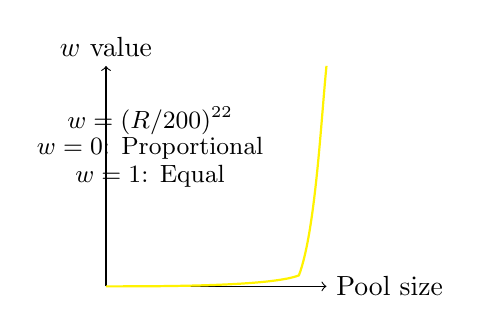
\begin{tikzpicture}[scale=0.7]
    % Axes
    \draw[->] (0,0) -- (4,0) node[right] {Pool size};
    \draw[->] (0,0) -- (0,4) node[above] {$w$ value};
    
    % Function
    \draw[yellow, thick] (0,0) .. controls (1,0) and (3,0) .. (3.5,0.2) .. controls (3.8,1) and (3.9,3) .. (4,4);
    
    % Annotations
    \node[align=left, font=\small] at (0.8,3) {$w = (R/200)^{22}$};
    \node[align=left, font=\small] at (0.8,2.5) {$w = 0$: Proportional};
    \node[align=left, font=\small] at (0.8,2) {$w = 1$: Equal};
\end{tikzpicture}
\end{column}
\end{columns}
\end{frame}

\begin{frame}{Longitudinal Study Results}
\begin{itemize}
    \item \textbf{Experiment 4:} Players participated in three consecutive games
    \begin{itemize}
        \item Games had random length with continuation probability
        \item Tested RL agent (M2) vs. proportional baseline
    \end{itemize}
    
    \item \textbf{Results:}
    \begin{itemize}
        \item RL agent generated larger surplus in all three games
        \item Surplus with RL agent \textit{increased} from game 1 to 3
        \item Surplus with proportional baseline \textit{decreased} over games
    \end{itemize}
    
    \item \textbf{Implication:} The RL mechanism becomes \textit{more} effective as participants gain experience with it
\end{itemize}
\end{frame}

\section{Evaluation}

\begin{frame}{Key Strengths of the Paper}
\begin{itemize}
    \item \textbf{Behavioral cloning as a powerful tool:}
    \begin{itemize}
        \item Creates incredibly accurate models of human behavior
        \item Enables rapid experimentation with different mechanisms
        \item Predictions from simulations match real-world outcomes
    \end{itemize}
    
    \item \textbf{Practical application of RL:}
    \begin{itemize}
        \item Solves a real socioeconomic problem
        \item Discovers non-obvious resource allocation strategies
        \item Shows how AI can inform (not just replace) human policymaking
    \end{itemize}
    
    \item \textbf{Interpretability:}
    \begin{itemize}
        \item Successfully distills complex RL policy into simple, explainable heuristic
        \item Demonstrates how complex AI solutions can inform simpler, practical policies
    \end{itemize}
\end{itemize}
\end{frame}

\begin{frame}{Limitations and Not-So-Good Parts}
\begin{itemize}
    \item \textbf{Generalizability concerns:}
    \begin{itemize}
        \item Participants from UK and USA only
        \item No demographic data collected to analyze group differences
        \item Stylized game may not fully translate to complex real-world scenarios
    \end{itemize}
    
    \item \textbf{Robustness issues:}
    \begin{itemize}
        \item Not tested across varying cultural contexts
        \item Limited exploration of parameter space (e.g., pool size, growth factor)
        \item Potential sensitivity to initial conditions
    \end{itemize}
    
    \item \textbf{Ecological validity:}
    \begin{itemize}
        \item Game differs from classic CPR problems (centralized allocation vs. free extraction)
        \item Controlled laboratory environment vs. complex real-world interactions
    \end{itemize}
\end{itemize}
\end{frame}

\section{Discussion}

\begin{frame}{Discussion}
\begin{itemize}
    \item \textbf{Behavioral clone vs. economic agent:}
    \begin{itemize}
        \item Behavioral clones excel at capturing actual human behavior
        \item Economic agents may perform better in theoretical models
        \item Trade-off: performance in static environment vs. adapting to policy shifts
    \end{itemize}
    
    \item \textbf{Equilibrium considerations:}
    \begin{itemize}
        \item What if we have RL agents designing mechanisms \textit{and} RL players participating?
        \item Potential "arms race" between mechanism design and player strategies
        \item Long-term stability of proposed solutions
    \end{itemize}
    
    \item \textbf{Broader implications:}
    \begin{itemize}
        \item Potential applications to public policy, institutional design
        \item Insights for resource allocation in organizational settings
        \item Parallel to Kuznets theory: inequality varies with resource abundance
    \end{itemize}
\end{itemize}
\end{frame}

\begin{frame}{Future Directions}
\begin{itemize}
    \item \textbf{Theory development:}
    \begin{itemize}
        \item Mathematical characterization of the discovered policies
        \item Formal connections to existing economic theories
    \end{itemize}
    
    \item \textbf{Extensions:}
    \begin{itemize}
        \item Testing across more diverse participant pools
        \item Exploring different variants of the CPR problem
        \item Applications to specific domains (environmental policy, public finance)
    \end{itemize}
    
    \item \textbf{Methodological advances:}
    \begin{itemize}
        \item Combining behavioral clones with cognitive/psychological models
        \item Integrating communication or partial communication between players
        \item Moving beyond strictly monetary incentives
    \end{itemize}
\end{itemize}
\end{frame}

\begin{frame}{Conclusion}
\begin{itemize}
    \item \textbf{Key contributions:}
    \begin{itemize}
        \item Demonstrated how deep RL can discover effective resource allocation mechanisms
        \item Created accurate behavioral models that predict human responses to different policies
        \item Derived an explainable heuristic that performs comparably to complex RL solution
    \end{itemize}
    
    \item \textbf{Broader impact:}
    \begin{itemize}
        \item Shows how AI can inform human policy-making in complex social dilemmas
        \item Provides insights on balancing efficiency and equality in resource allocation
        \item Offers a framework for studying similar problems in other domains
    \end{itemize}
    
    \item \textbf{Take-home message:} Deep RL can reveal non-obvious but effective strategies for promoting sustainable collective behavior
\end{itemize}
\end{frame}

\begin{frame}{References}
\begin{itemize}
    \item Koster, R., Pîslar, M., Tacchetti, A., Balaguer, J., Liu, L., Elie, R., Hauser, O.P., Tuyls, K., Botvinick, M., \& Summerfield, C. (2025). Deep reinforcement learning can promote sustainable human behaviour in a common-pool resource problem. \textit{Nature Communications}, 16(2824).
    
    \item Koster, R., et al. (2022). Human-centred mechanism design with democratic AI. \textit{Nature Human Behaviour}, 6, 1398-1407.
    
    \item Ostrom, E. (1991). Governing the Commons: The Evolution of Institutions for Collective Action. Cambridge University Press.
    
    \item Fehr, E., \& Gächter, S. (2002). Altruistic punishment in humans. \textit{Nature}, 415, 137-140.
\end{itemize}
\end{frame}

\end{document}